% Our document type specification.
\documentclass[a4paper,14pt]{article}

% this changed from the font to the default sans serif font
%\renewcommand{\familydefault}{\sfdefault}
% This is often sufficient, but geometry
% allows one to more fully use a page.
\usepackage[myheadings]{fullpage}
\usepackage[T1]{fontenc}
\renewcommand{\familydefault}{\sfdefault}
%\usepackage{helvet}
% Allows us to manipulate header and footer data.
\usepackage{fancyhdr}
\pagestyle{fancy}
%\rhead{Wayne Buchner, 6643140} % Header right.
%\lhead{Case Study: Swinburne Bookshop Co-operative} % Header left.
\rfoot{} % Footer right.
\lfoot{} % Footer left.

% A generally useful package for
% presenting maths-related things.
%\usepackage{amsmath}
%\usepackage{metre}
%\usepackage{parskip}
% Provides commands for printing text
% in the exported document as it
% appears in the LaTeX document.
\usepackage{verbatim} 
\usepackage{harvard}
\usepackage{url}
% for multiple rows in tables
\usepackage{multirow}

\usepackage{caption}

% Lets one modify the paragraph
% settings of the document.
\usepackage{parskip}
\setlength{\parskip}{0pt}
\setlength{\parindent}{0pt}

% Used to import images for figures.
\usepackage{graphicx}
% Uncomment to add background images!
%\usepackage{eso-pic}
%\AddToShipoutPicture{%
%\put(0,0){\includegraphics{background.pdf}}%


\usepackage{sidecap}
\usepackage{float}
\usepackage{wrapfig}
\floatstyle{boxed} 
\restylefloat{figure}
% A supplementary package for listings.
\usepackage{fancyvrb}

% Defines a number of colours.
\usepackage[usenames,dvipsnames]{color}
%\usepackage{titlesec}
%\definecolor{sectionred}{rgb}{199,55,44}
%\titleformat{\section}
%{\color{sectionred}\normalfont\Large\bfseries{\thesection}{1em}{}

\usepackage{sectsty}
\sectionfont{\sffamily\underline}

% Allows us to include code listings.
% The following lines configure settings
% for this package.
\usepackage{listings}
\lstset{language=[Objective]C, breakindent=40pt, breaklines}
\lstset{ %
basicstyle=\footnotesize,
breaklines=true,
breakatwhitespace=false
}
\lstdefinelanguage[FPC]{Pascal}[Standard]{Pascal}
 {%
	morecomment=[l]//,%
  	morekeywords={uses,external,cdecl,export,%
	forward,global,module,nil,operator,overload,%
	priority,sum,type,use,dispose,mark,page,%
	release,eof,eoln,ord,pos,pred,rval,succ,%
	result,interface,implementation,unit}%
 }%
\lstset{keywordstyle=\color{Blue}}
\lstset{commentstyle=\color{OliveGreen}}
\lstset{stringstyle=\color{BrickRed}}
\lstset{basicstyle=\scriptsize \sffamily}
\lstset{captionpos=t}
\lstset{frame=trbl}
\lstset{fancyvrb=true}
\lstset{numberstyle=\footnotesize}
\lstset{showstringspaces=false}
\lstset{tabsize=2}
\lstset{language=[FPC]Pascal}
\lstset{captionpos=b}

% Applies an effect to captions; in
% this case our listing captions.
\usepackage{caption}
\captionsetup[lstlisting]{labelfont=bf}

% Provides nicer quotation marks for code.
\usepackage{upquote}

% Used to change row spacing in tables.
\usepackage{array}

% Provides extra options for appendices.
\usepackage{appendix}

% Supplies linking capabilities.
\usepackage{hyperref}
\hypersetup{
    colorlinks,
    citecolor=black,
    filecolor=black,
    linkcolor=black,
    urlcolor=blue
}

% Allows us to use glossaries.
\usepackage{glossaries}
\newglossaryentry{sbs}{name = Swinburne Bookshop Co-operative, description = Swinburne Bookshop Co-operative}
\newglossaryentry{gui}{name = Graphic User Interface, description = Graphic User Interface}
\newglossaryentry{mvc}{name = Model View Controller, description = Model View Controller}

%\newacronym{oop}{OOP}{Object Oriented Programming}
%\newacronym{gui}{GUI}{Graphic User Interface}
%\newacronym{mvc}{MVC}{Model View Controller}
\makeglossaries
% Glossary Items


\makeglossaries
% Separate our lines.
\linespread{1.2}
\setcounter{page}{0}
\title{Research Report\\Use of objects in Graphic User Interfaces in Cocoa and Java Swing Foundation classes}
\author{Wayne Buchner,6643140}
\date{13-11-2011}

\begin{document}

\ifpdf
\DeclareGraphicsExtensions{.pdf, .jpg, .tif}
\else
\DeclareGraphicsExtensions{.eps, .jpg}
\fi

\maketitle
\thispagestyle{empty}
\newpage
\tableofcontents
\newpage

\section{Introduction} % (fold)
\label{sec:introduction}
The \gls{gui} allows the user to interact with a program by manipulating properties of objects there by sending information from the View to the Controller. Both Objective C and Java accomplish this in similar ways. This research report focuses on the differences in producing \gls{gui}s using Objective C's Cocoa and Java's Swing packages. Inherently the greatest point of difference in developing on the aforementioned platform is Java Swing's ability to be a truly cross platform framework \cite{nla.cat-vn3060178}. Where as Apples Cocoa is a powerful platform centric framework constructed purely for the Mac OS and iOS platforms. This provides a focused set of frameworks. 

%
% NEED TO FIND THE RIGHT SECTION FOR THIS
\citeasnoun{Dias2011} states that writing code can be a daunting experience for novice programmers and that designing an interface using direct manipulation of objects is a powerful learning tool to what was once a steep learning curve. Research undertaken for this document will provide proof that advances in \gls{gui} builders significantly reduce code writing time, increasing efficiency and reduce errors. Removing unnecessary debugging time from the development lifecycle by reducing errors and increasing code quality as GUI builders improve, may reduce development times and allow developers to concentrate on other areas. Tests results generated for this paper are the results of timed tests between Apple's native integrated development environment, XCode and Oracles Netbeans. Results are the comparison in improvements to code completion and build times.  
%

\textbf{Section \ref{sec:graphic_user_interface_architecture}} will introduce the \gls{gui} architecture and explain at a high level the structure of the class hierarchies including an introduction to the Model View Controller (MVC) principals. \textbf{Section \ref{sec:view_hierarchy_in_cocoa}} and \textbf{\ref{sec:view_hierarchy_in_swing}} introduce and display objects of related view classes. \textbf{Section \ref{sec:hello_world}} compares differences at the highest level between a Hello World program while \textbf{Section \ref{sec:simple_calculator}} discusses and explains points of difference between a more complex program, and \textbf{Section \ref{sec:results}} outlines the results of the Simple Calculator program tests.
% section introduction (end)

\section{Graphic User Interface Architecture An Introduction} % (fold)
\label{sec:graphic_user_interface_architecture}
A \gls{gui} allows the user to interact with a system. A well designed interface should leverage a users existing knowledge there by improving the effectiveness of the users interaction. Both Cocoa and Swing allow for the layering of objects to be built in a hierarchical manor in order for the user to perform tasks, or in programming terminology trigger events. Although they achieve this in different ways, the semantics are minute in terms of actual designing, where Cocoa generally moved towards a design process based more on WYSIWIG allowing for more productive workflow, other development languages have been slow to implement or follow this lead. Developing a \gls{gui} in Swing can be achieved either through a plain text file containing the code for a window or via a WYSIWIG editor found in IDE's such as BlueJay, Netbeans or Eclipse.

Both platforms isolate the view from the data by implementing the \gls{mvc} design pattern and the similarities do not end there. Both inherit all core functionalities from a root Object class, NSObject for Cocoa and the JComponent class for Swing. Briefly, although the terminology may be different, both frameworks create an interface in a similar manor.


\begin{table}[H]
\centering
\begin{tabular}{l}
\includegraphics[scale=1.0]{tableSimilarClasses.eps}
\end{tabular}
\caption{Average time of 20 build cycles for a simple Hello World Program}
\label{table:tableSimilarClasses}
\end{table}


Table \ref{table:tableSimilarClasses} outlines that both platforms fundamentally build a \gls{gui} using similar constructs. The class names may be different however the principal behind them are similar. Where Java Swing endeavors to supply a cross platform framework, Cocoa is tailored to the MacOS and iOS platforms offering a more rigid, extensible framework build foremost with the platforms specifications but most importantly built to take advantage of the platforms hardware as well.. 

\section{View Hierarchy in Cocoa} % (fold)
\label{sec:view_hierarchy_in_cocoa}
Figure \ref{fig:cocoaHierarchy} shows Cocoa's UIKit Class Hierarchy. Note that all objects inherit directly from the root class of NSObject. Also being more platform specific it has platform centric objects targeted at specific hardware devices. Building a \gls{gui} using Cocoa has been further simplified by the employment and development over countless iterations of the Integrated Development Environment, XCode. XCode's interface builder offers detailed information on objects and offers only objects appropriate for use in the particular project, saving the developer time implementing unsupported user interface elements. As an aside, the newest iteration of XCode allows for storyboarding of windows to further simplify navigation between Views.


\begin{figure}[H]
\centering
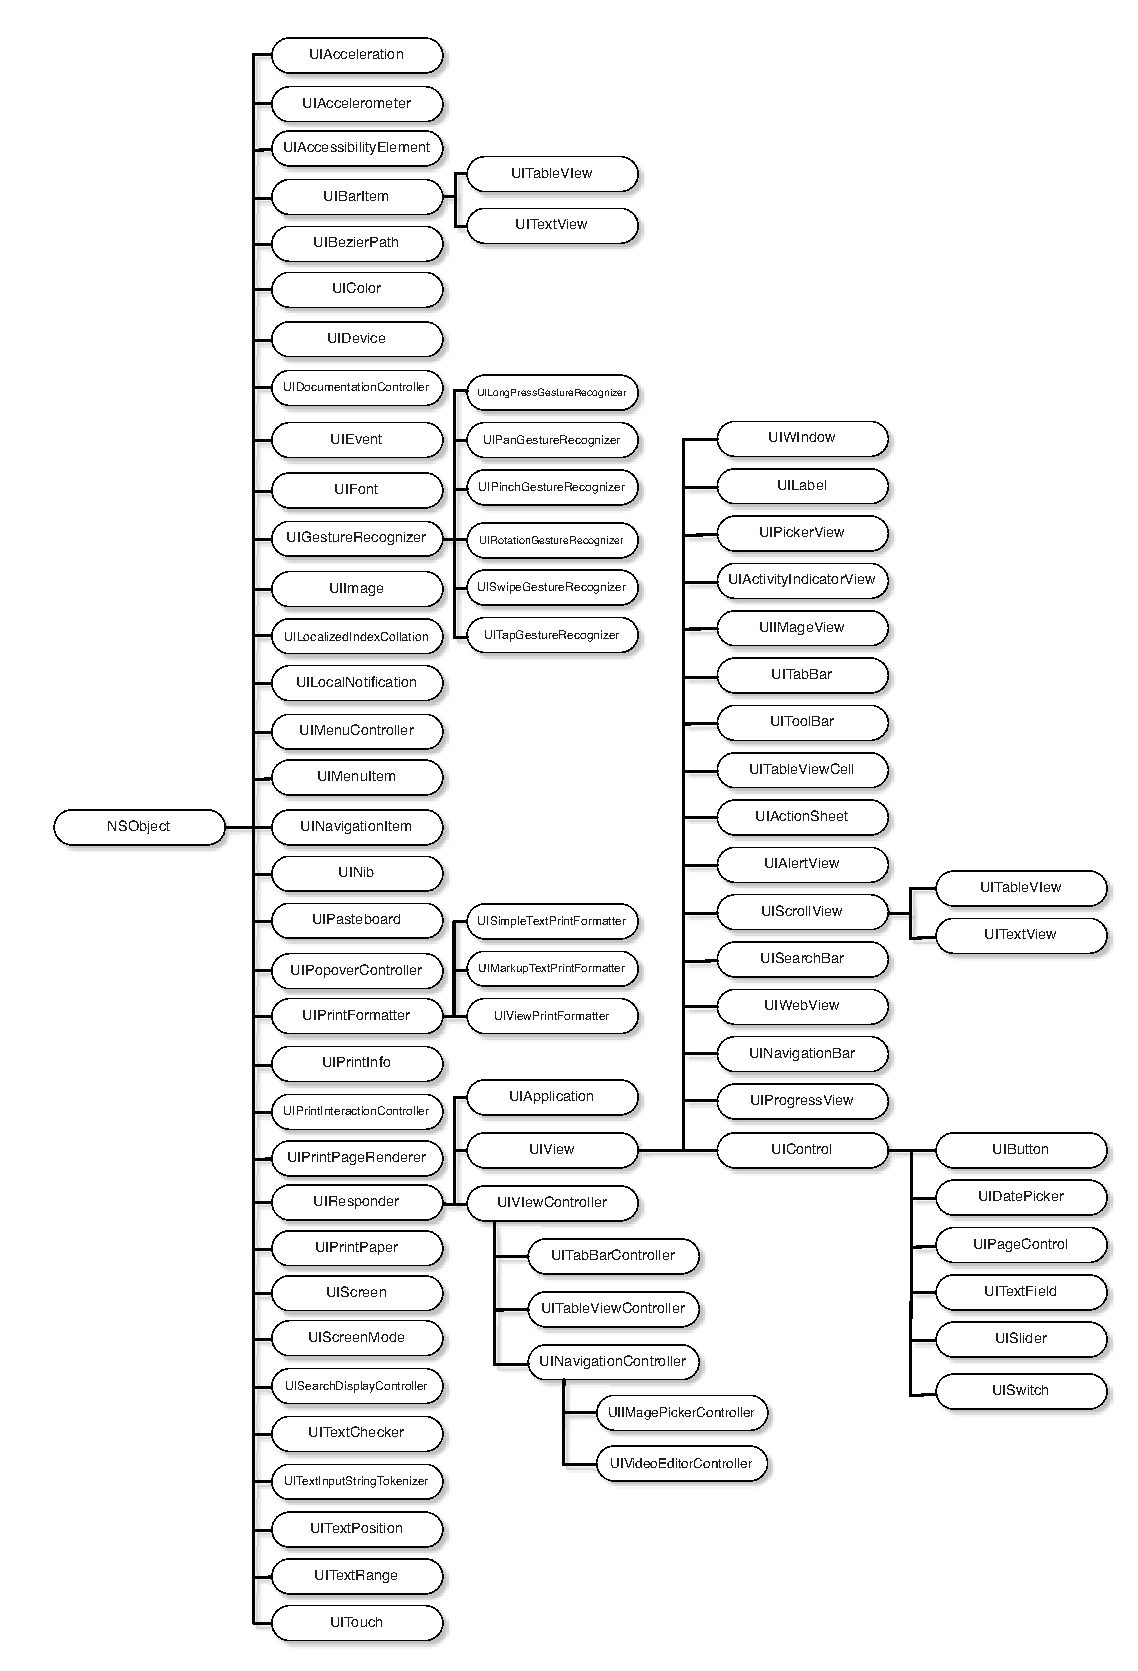
\includegraphics[scale=0.80]{UIKitClassHierarchy.eps}
\caption{Cocoa UIKit Class Hierarchy. \protect\citeasnoun{Apple2010a} }
\label{fig:cocoaHierarchy}
\end{figure}
% subsection view_hierarchy_in_cocoa (end)

\section{View Hierarchy in Swing} % (fold)
\label{sec:view_hierarchy_in_swing}
In Figure \ref{fig:swingHierarchy} you can see that Swing's hierarchy is configured only slightly differently, with JComponent inheriting from the Container class, whose root class is Object. Java Swing is a lightweight framework built on top of Java's awt framework. Due to it's completely Java construction it can be easily mixed with other Java Component class objects such as standard Java AWT labels, text fields and scrollbars.


\begin{figure}[H]
\centering
\includegraphics[scale=0.8]{Java1.png}
\caption{Swing Class Hierarchy. \protect\citeasnoun{Oracle2010}}
\label{fig:swingHierarchy}
\end{figure}
% subsection view_hierarchy_in_swing (end)

%
%  TALK A LITTLE ABOUT DYNAMIC STUFF
%
%

\section{Hello World} % (fold)
\label{sec:hello_world}
Moving from text based user interaction to a \gls{gui} the understanding of how input is received changes. A programmer must shift from taking the result of a direct prompt to listening for user interactions. This is called event based programming and that is how \gls{gui}'s work. Both Swing and Cocoa work in this manor. In both frameworks, \textbf{Event Listeners} respond to interaction with specific elements of the UI.



\begin{figure}[H]
\centering
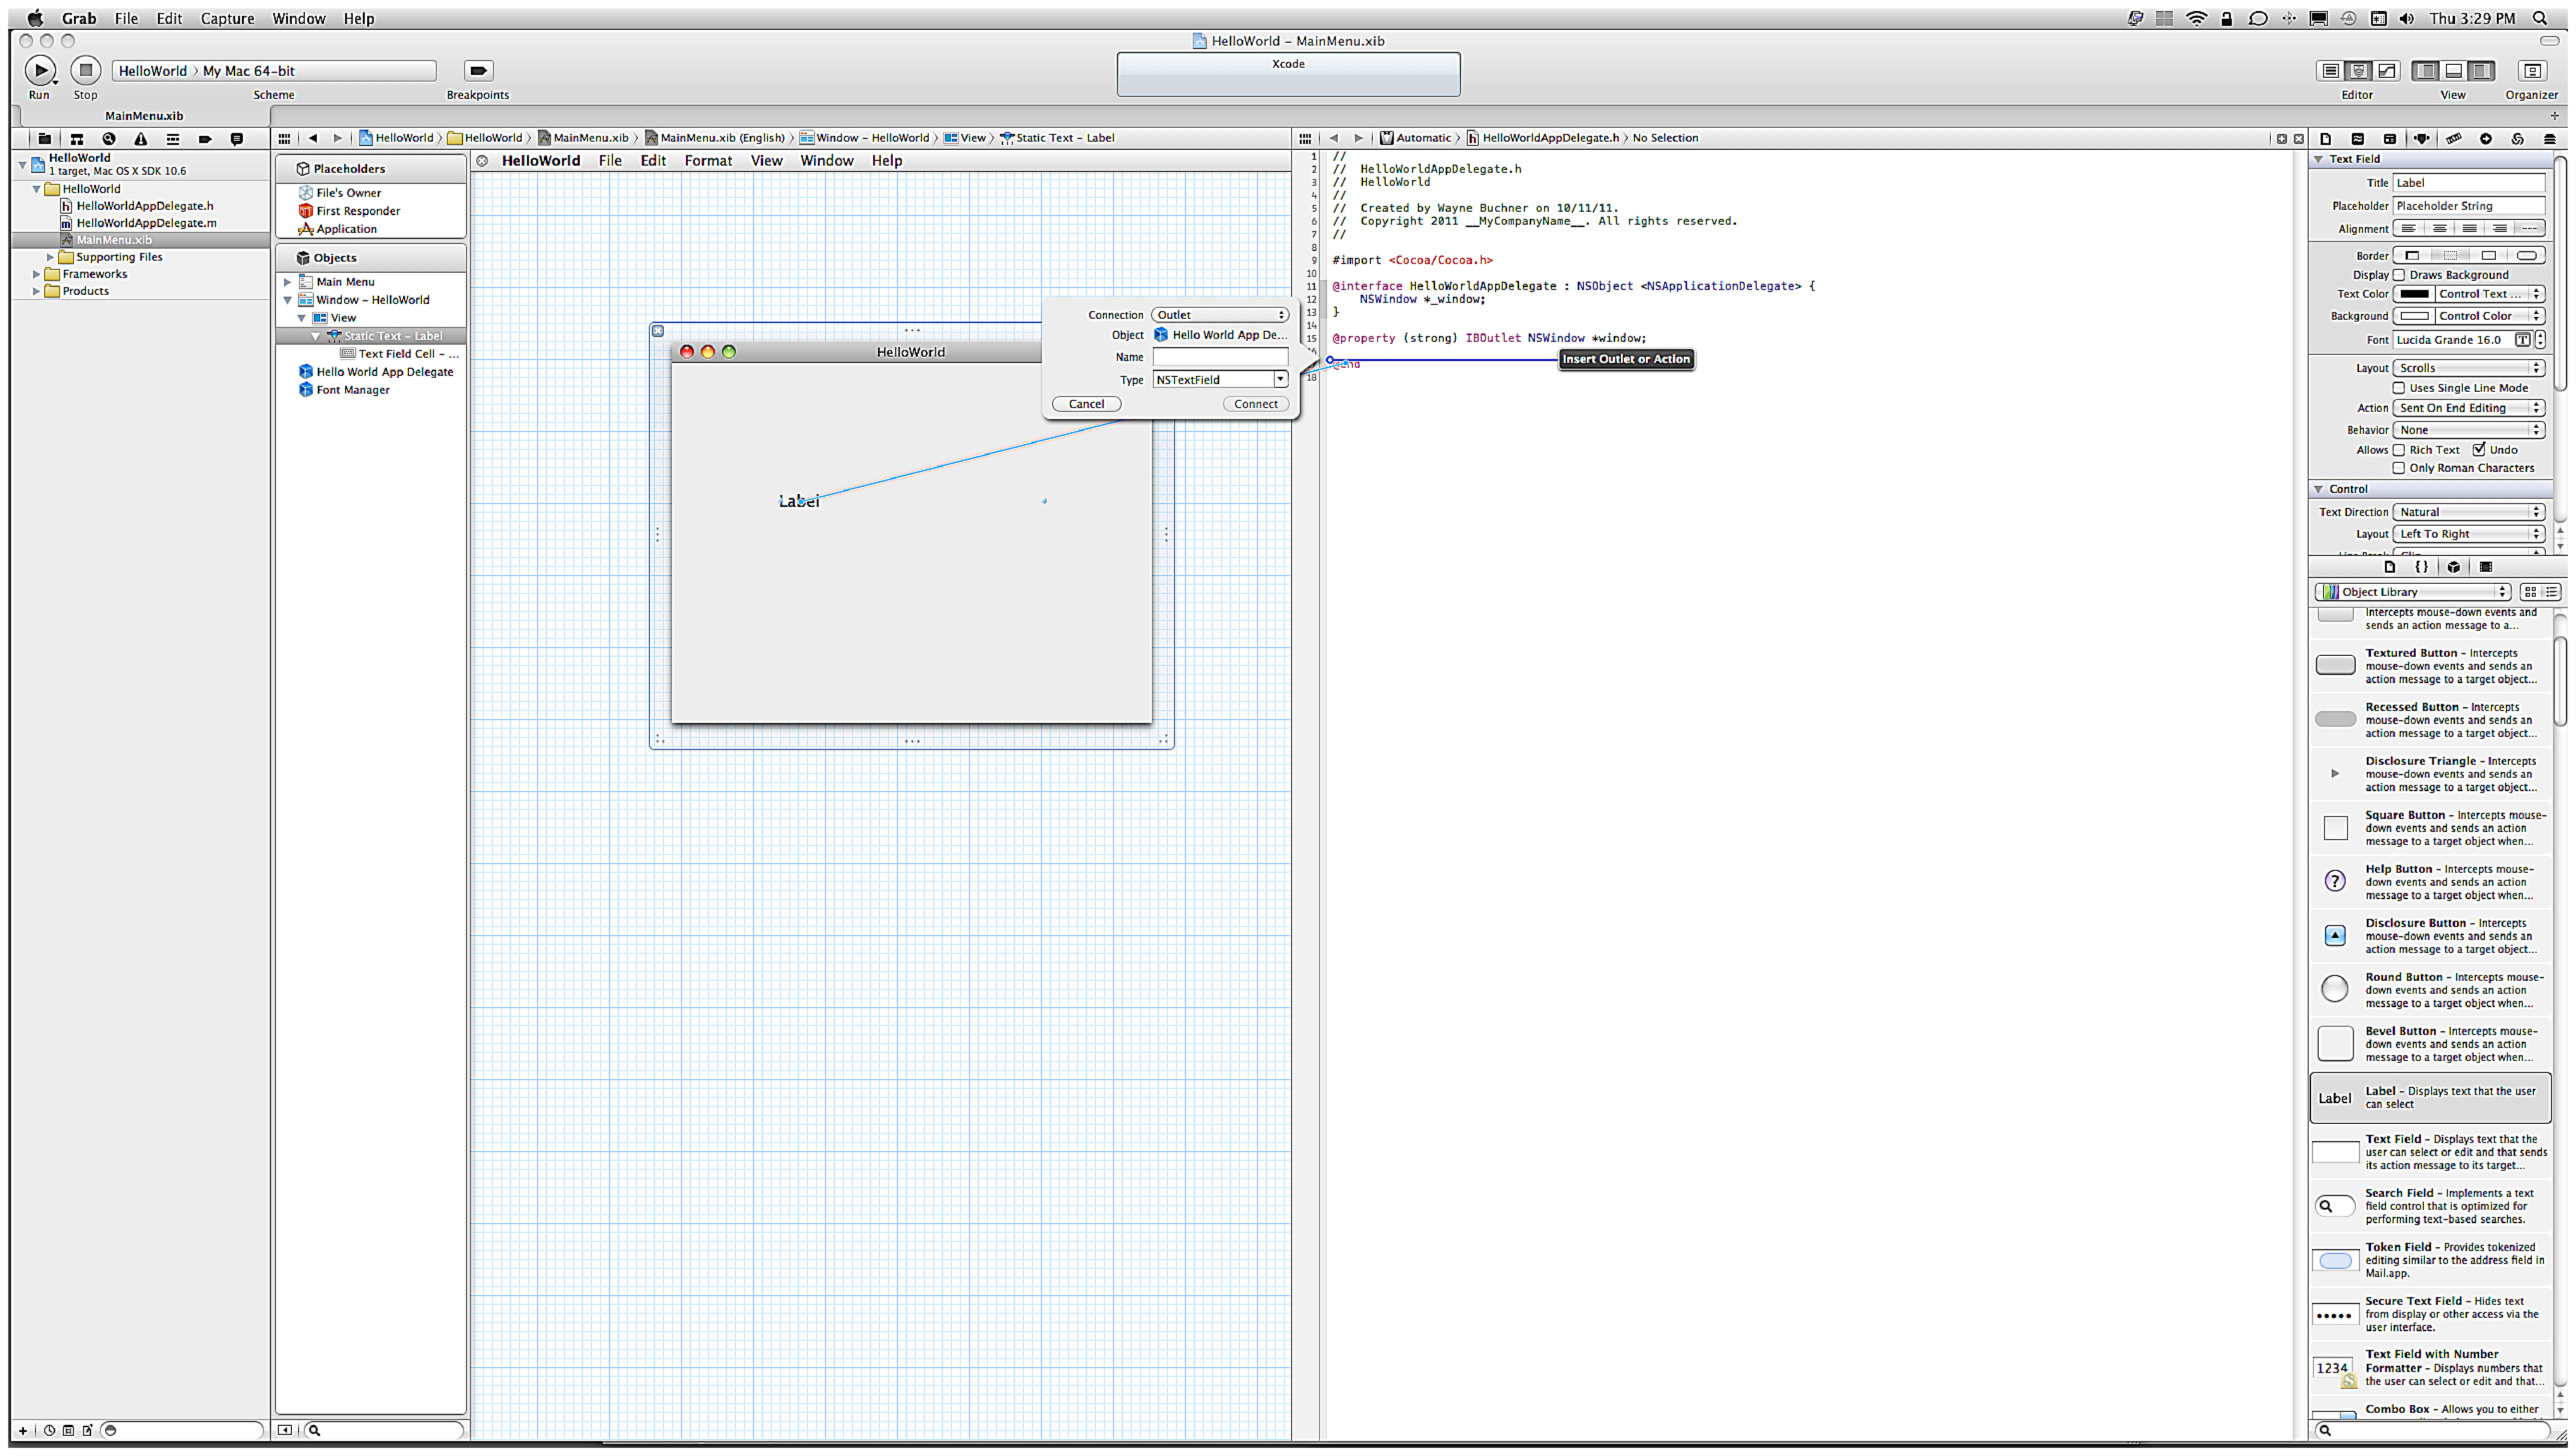
\includegraphics[scale=0.17]{HelloWorldLabelHookUp.eps}
\caption{Interface Builder, XCode 4.1}
\label{fig:interfaceBuilder}
\end{figure}

Figure \ref{fig:interfaceBuilder} shows the simplicity of \textbf{Hooking Up} an object created in interface builder to the view controller. Once an object has been created and Hooked up to a view controller or a delegate, it then becomes available to manipulate throughout the class via generated code placed directly into the corresponding header and implementation files. XCode places the correct getter and setter methods for the properties of the object via the @synthezise declaration. Java's design view works in a similar way Figure \ref{fig:netbeans} shows the Design View for a Java Swing window. Selecting the object in the design view and adding an \textbf{Event} places an event listener method into the class ready for code in a similar way that XCode places the method into the implementation file. 

Constructing the user interface with the assistance of a \gls{gui} builder proved extremely fast on both platforms. Table \ref{table:buildTimes} compares the user interface construction and build times for the test Hello World program using hand coding versus the IDE's assisted user interface builder. Based on the results constructing the Hello World program, developing time for a complex user interface like the interface shown in Figure \ref{fig:swintrekui} will be dramatically improved using an \gls{gui} builder. The figures in Table \ref{table:buildTimes} would indicate there is no noticeable difference in build time for either platform when comparing between the programs hand coded versus auto generated code. Where the figures return an indication of difference lie in the ability to efficiently design and layout a user interface.

\begin{figure}[H]
\centering
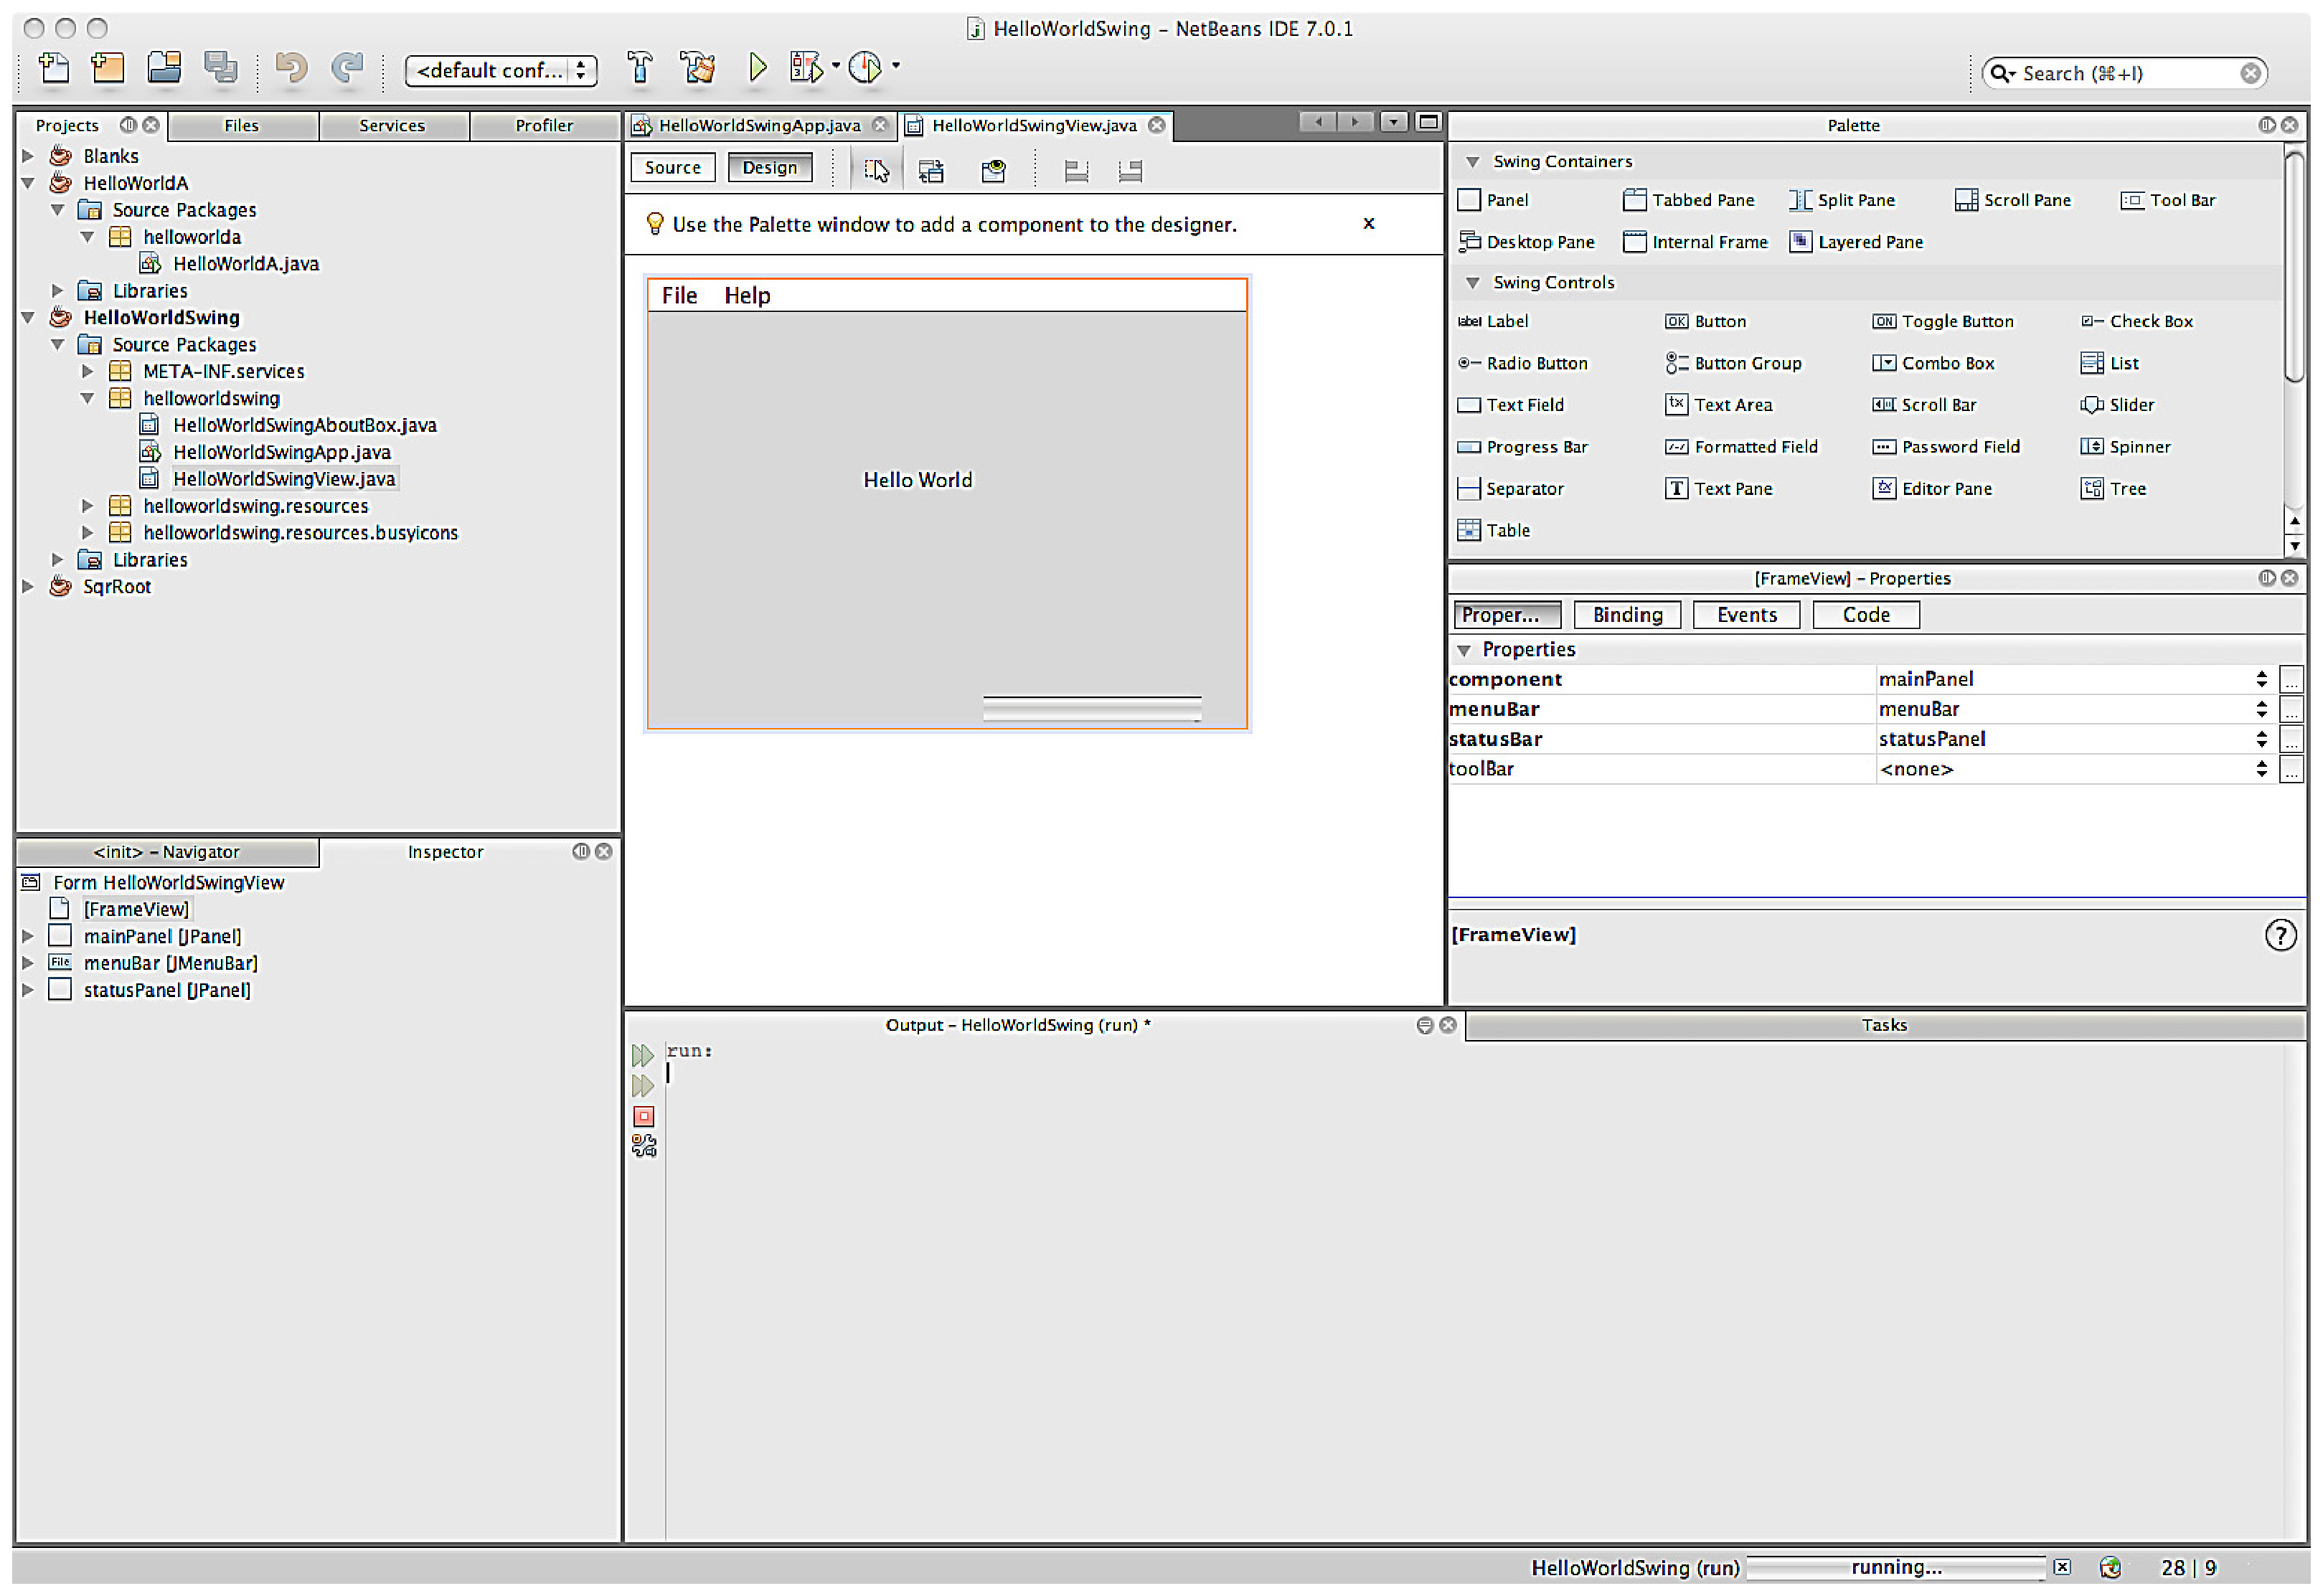
\includegraphics[scale=0.29]{netbeans.eps}
\caption{Design View, NetBeans 7.01}
\label{fig:netbeans}
\end{figure}

\begin{table}[here]
\centering
\begin{tabular}{l}
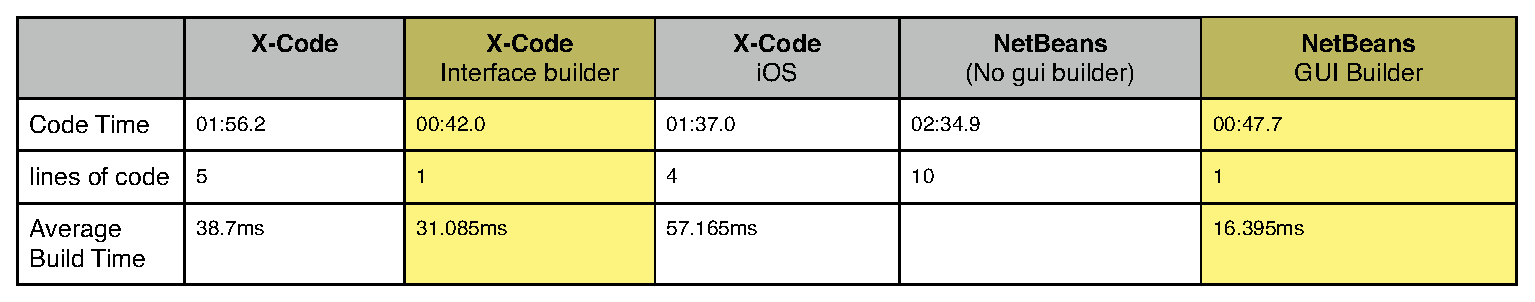
\includegraphics[scale=0.62]{TableBuildCompares.eps}
\end{tabular}
\caption{Average time of 20 build cycles for a simple Hello World Program}
\label{table:buildTimes}
\end{table}

\begin{figure}[H]
\centering
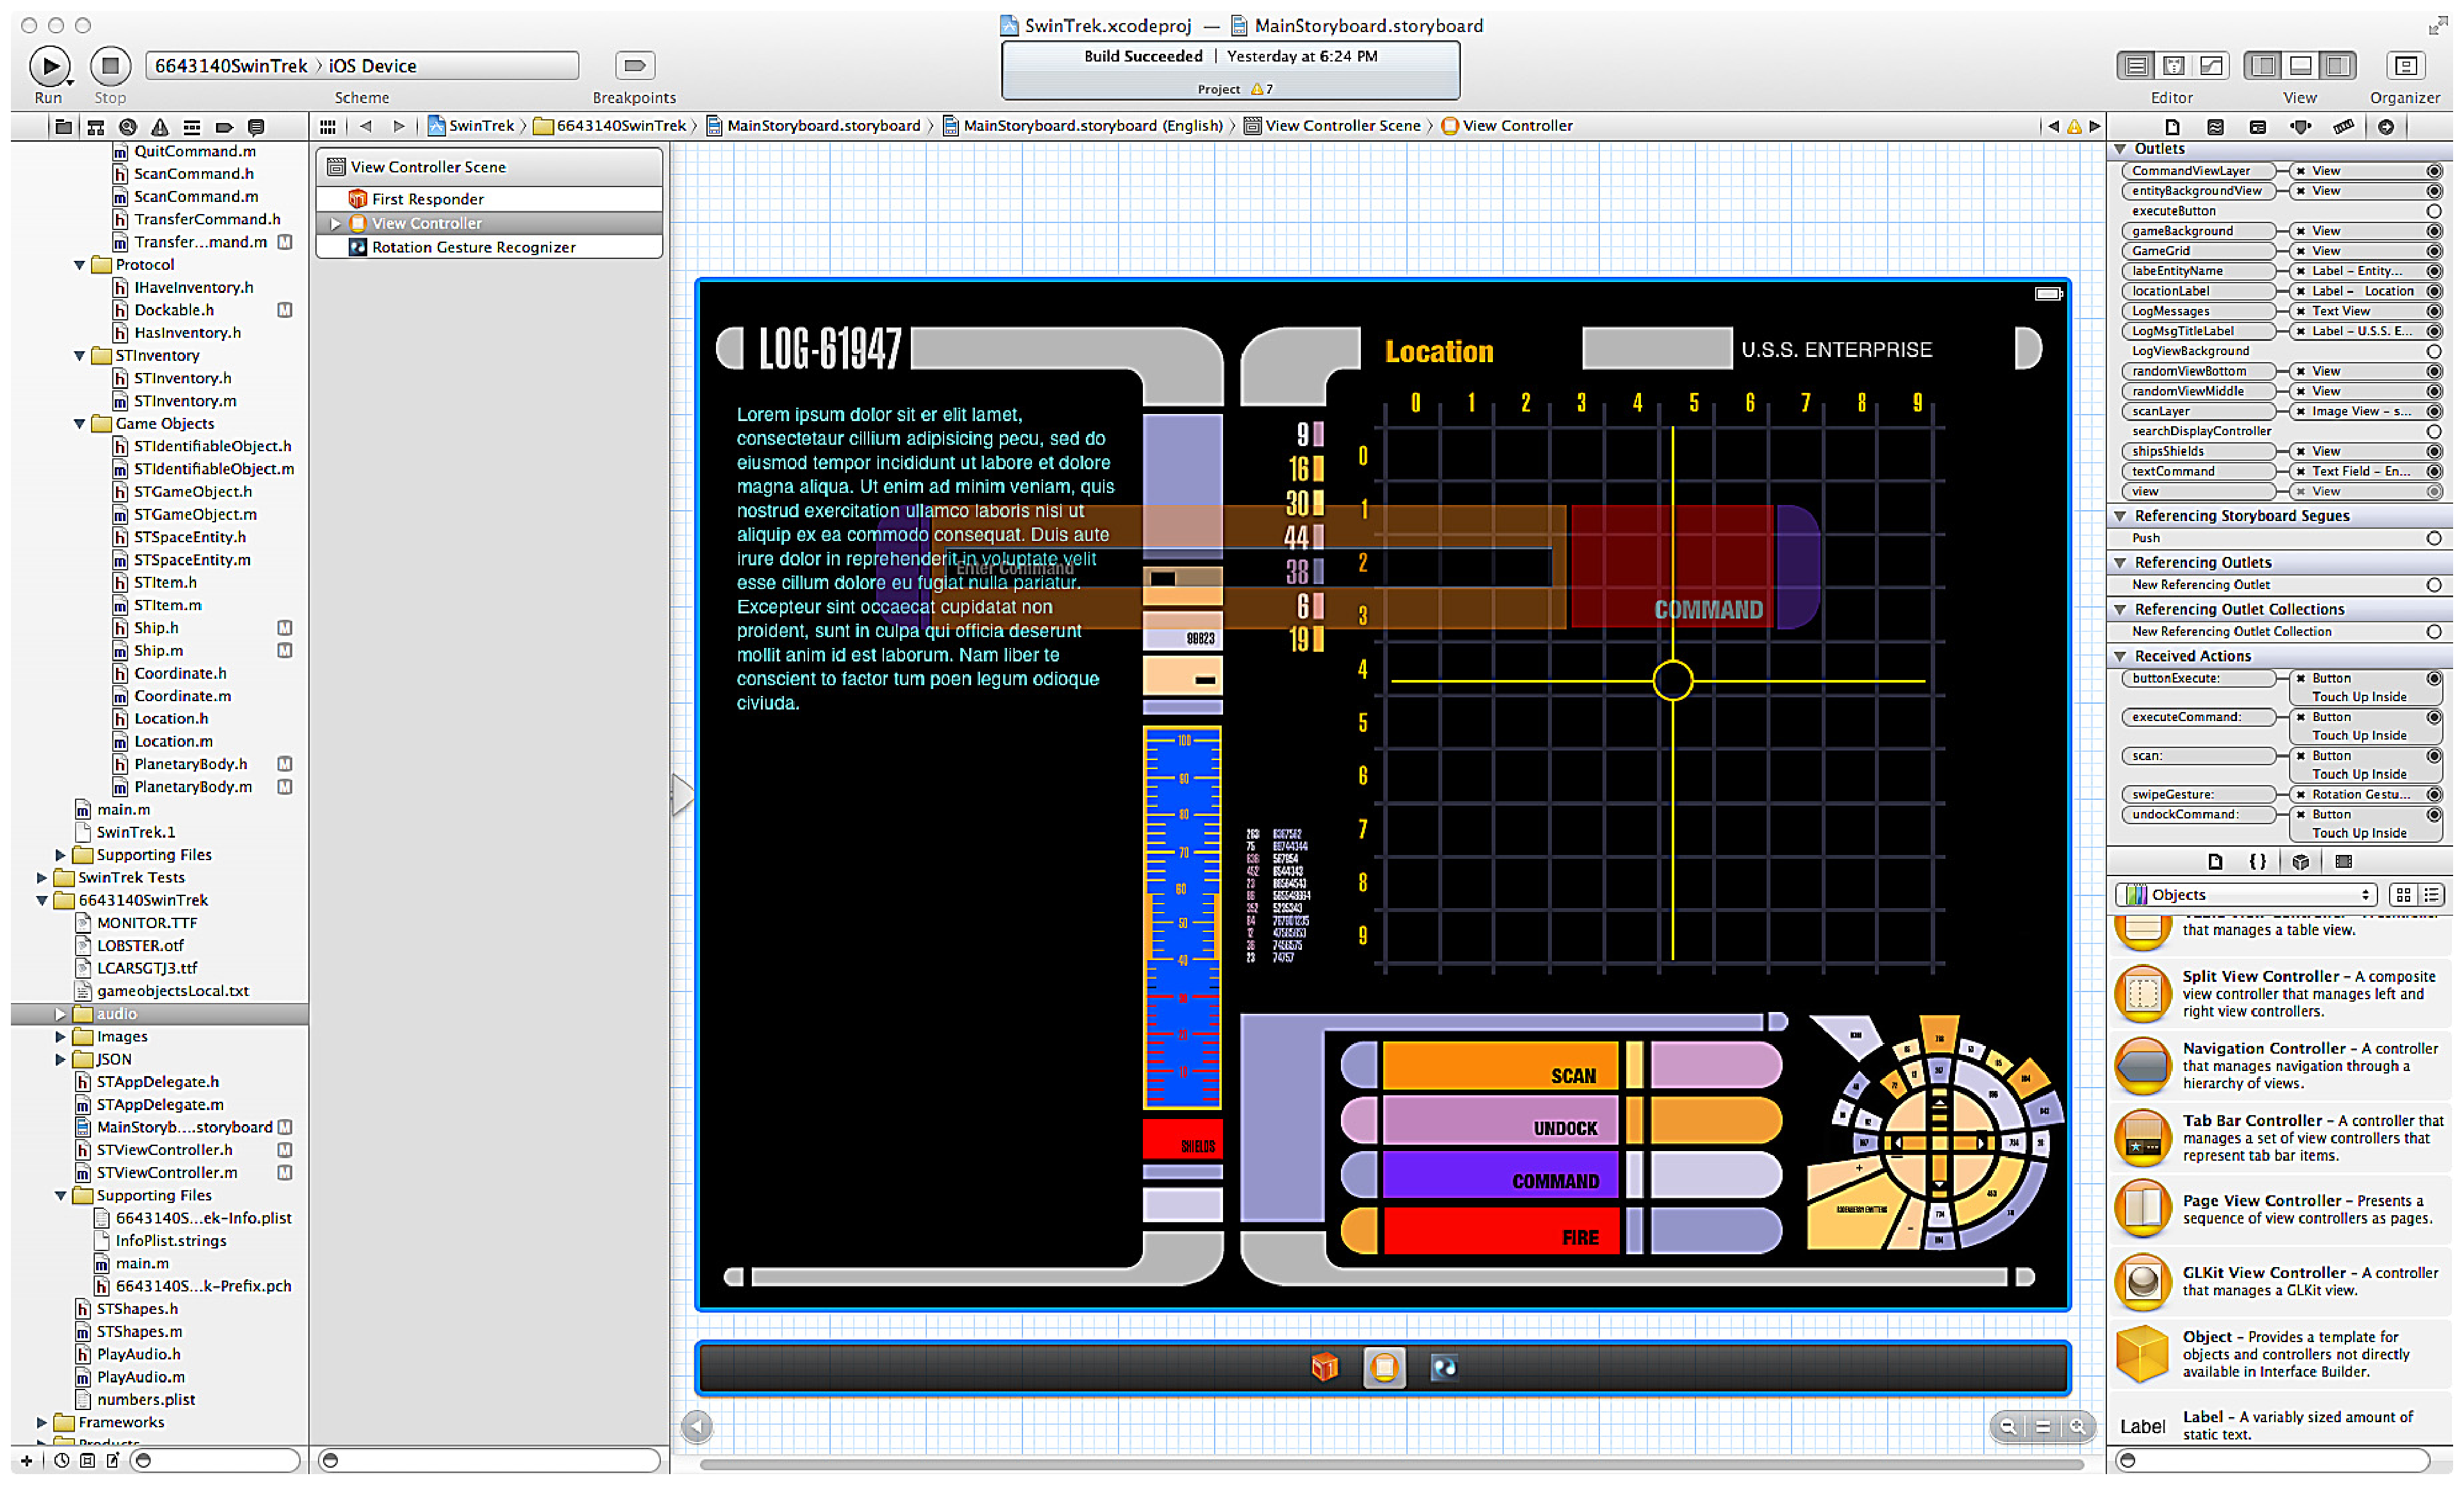
\includegraphics[scale=0.24]{swintrekuserinterface.eps}
\caption{SwinTrek User Interface, XCode}
\label{fig:swintrekui}
\end{figure}

\textbf{Getting} and \textbf{Setting} objects properties created using GUI builders operate similarly in both platforms. Differences across the platforms are syntactical and reserved to either taking the shortcut in XCode and allowing it to synthesize these properties values for you, or writing the getters and setter code as you would in the same way in Java. The benefit of XCode is the ability to change these post GUI build where as in NetBeans changing a property created by the GUI, the name perhaps or removing it must be done through the GUI builder.
% subsection hello_world (end)

\section{Simple Calculator} % (fold)
\label{sec:simple_calculator}
Further testing the hypothesis that XCode is a more efficient IDE as offered in section \ref{sec:hello_world} is proven in this section. Results of the Hello World program shown in \ref{sec:hello_world} are further collaborated by constructing and testing a more complex program. A calculator that adds or subtracts two numbers in both Objective C and Java would be used to as further evidence. The devised test is to build four programs, a hand Coded Calculator and a Calculator created with the help of the IDE's interface builder over both platforms. This process was timed recording Build and run sequences, lines of code required and average errors per build. The results for building the simple calculators can be seen in Table \ref{table:simplecalc}. 
\begin{table}[H]
\centering
\begin{tabular}{l}
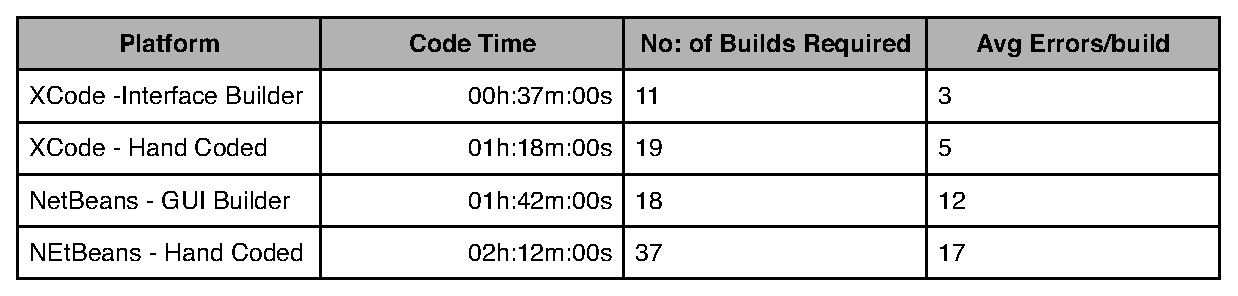
\includegraphics[scale=0.65]{simplecalculator.eps}
\end{tabular}
\caption{Recorded Statistics for the Simple Calculator Test}
\label{table:simplecalc}
\end{table}
Apart from a dramatic difference in build time, laying out objects in XCode was a more efficient process. \citeasnoun{nla.cat-vn3060178} state that the most compelling reasons for using GUI builder for an application with even moderate complexity, is for efficiency. XCode's interface builder offers more affordance for the programmer and is far simpler to initialize parameters inside the IDE than NetBeans. Another point of difference where XCode allows free reign for placement of objects onto the window, Java utilizes a layout manager to specify and control the layout of objects on a JPanel or JContainer \cite{nla.cat-vn3060178}. By default Java places objects into a FlowLayout unless specified otherwise. Although object properties can be altered, Java's documentation says that it's layout manager has the final say on the size and position on components within containers \cite{Oracle2011}. Other layout managers can be initialized if required, they are:
\begin{enumerate}
		\item BorderLayout
		\item CardLayout
		\item FlowLayout
		\item GridBagLayout
		\item GridLayout
\end{enumerate}

\begin{figure}[H]
\centering
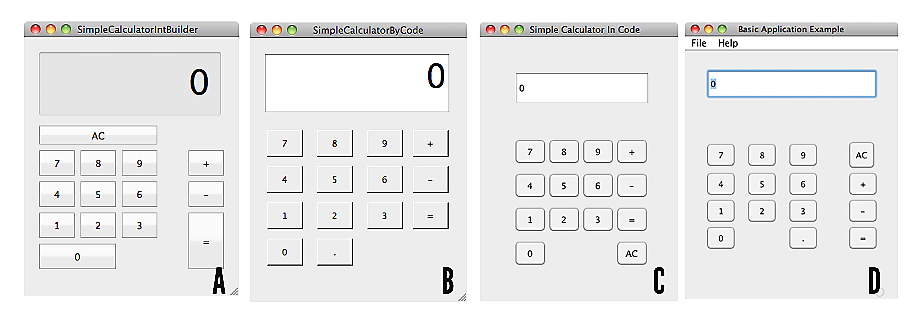
\includegraphics[scale=1.0]{Calculators.eps}
\caption{Four Test Calculators}
\label{fig:calculators}
\end{figure}
Figure \ref{fig:calculators} shows the layouts of the calculators produced for the tests.
\begin{enumerate}
\item Calculators labeled A through B:
	\begin{itemize}
	    \item A: Built in XCode using Interface Builder
	    \item B: Built in XCode, hand coded.
	\end{itemize} 
	\item Calculators labeled C through D:
		\begin{itemize}
		    \item C: Built in NetBeans using using the IDE's Interface Builder and Java Swing Packages.
		    \item D: Built in NetBeans, hand coded using Java Swing Packages.
		\end{itemize}
\end{enumerate}

\begin{table}[H]
\centering
\begin{tabular}{l}
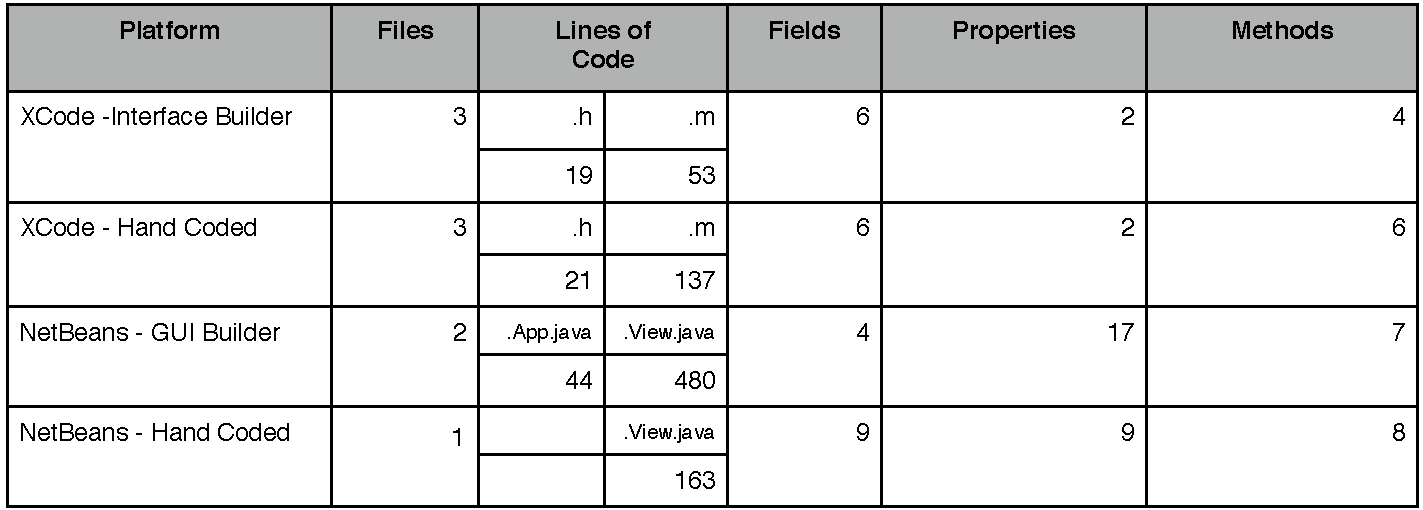
\includegraphics[scale=0.6]{FileComparisons.pdf}
\end{tabular}
\caption{Simple Calculator Comparison Results}
\label{table:calccompare}
\end{table}
Code practices for each platform were strictly adhered to. This allowed for the best possible comparison between the two platforms. It is clear to see from Table \ref{table:calccompare} that XCode produces the least amount of code to accomplish the result. Not only does this conform well with ISO9126(1992) standards of Good Programming Practices, future maintenance of the Objective-C's calculators will be easier than the auto generated Java code of 480 lines. Java/NetBeans creates 905\% more code for it's auto generated calculator and 118\% more for the hand written code. The reasons for these are outlined in Section \ref{sec:results}.

\section{Results} % (fold)
\label{sec:results}

% subsection results (end)
Objective-C allows for the multiple use of instance variable names which allows for greater code flexibility when creating dynamic object instances such as buttons. Java insists on creating each object instance with a unique name. Creating a button in Objective-C entailed one method shown in Listing \ref{generateButtonObj}. When called by the class it instantiated an instance of NSButton, added all the required properties to initialize the button and was added to the view. Further evidence of this can be seen in Figure \ref{fig:classDiagrams} which shows class diagrams for each program. The Class diagrams show the Calculator created with the assistance of XCodes Interface Builder creates the most succinct class diagram and generates the cleanest code from which to extend.
\begin{figure}[H]
\centering
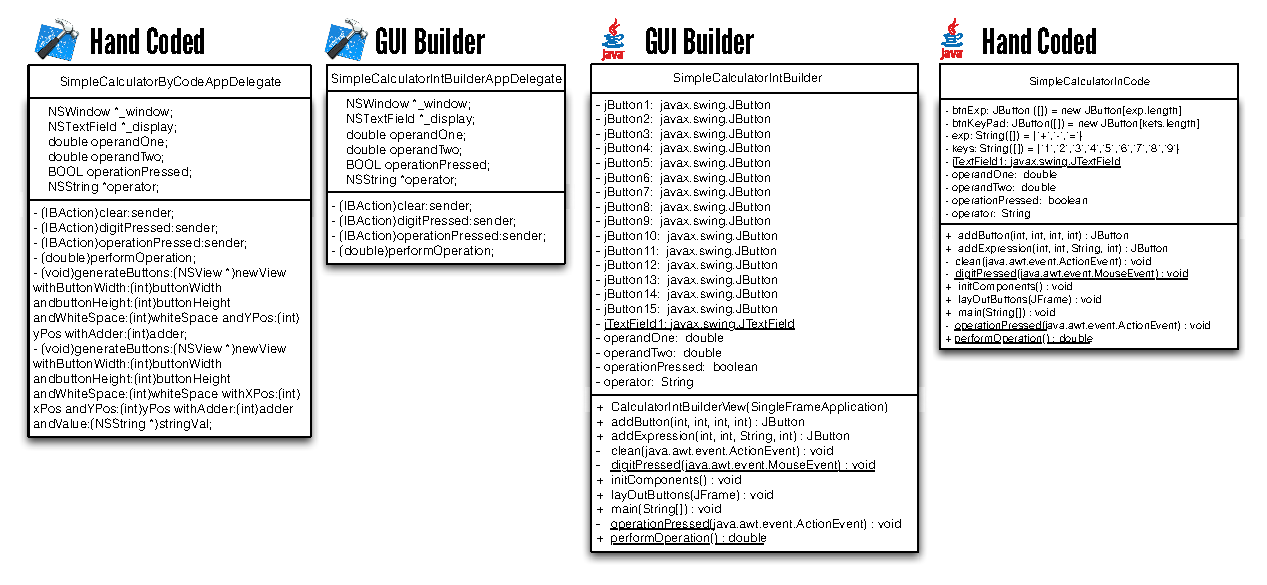
\includegraphics[scale=0.75]{ClassDiagrams.eps}
\caption{Class Diagram Comparison}
\label{fig:classDiagrams}
\end{figure}
\begin{lstlisting}[caption={Create Button - Objective-C},language=C,label=generateButtonObj,]
- (void)generateButtons:(NSView *)newView withButtonWidth:(int)buttonWidth andbuttonHeight:(int)buttonHeight andWhiteSpace:(int)whiteSpace withXPos:(int)xPos andYPos:(int)yPos withAdder:(int)adder andValue:(NSString *)stringVal
{
    NSButton *button = [[[NSButton alloc] initWithFrame:NSRectFromCGRect(CGRectMake(xPos, yPos , buttonWidth, buttonHeight)) ]autorelease];
    [button setTitle:stringVal];
    [newView addSubview:button];
    [button setAction:@selector(operationPressed:)];
}
\end{lstlisting}
Alternatively NetBeans auto generated code insisted on creating a field for each button with a unique name. The version of the Calculator built using NetBeans interface builder created fifteen buttons as fields. Each Button created it's own Event Handler which needed to be deleted and rethreaded to a single event handler where the event could be determined and the button recast to a new object where the objects properties could be manipulated.
This was again different in the hand coded Java Calculator. The method shown in Listing \ref{addButtonJava} emphasizes the difference. An array of Strings was used for the instance name, syntactically the code is far more verbose. Due to the necessity of requiring additional methods to create my keypad it is necessary to return the button created out of this method for use by another method that added the object to the view, titles \textbf{layOutButtons}, seen in Listing \ref{layOutButtons}.
This is due to the fact that Objective-C is creating a pointer to the referenced object created as the property, for example the button is allocated on the heap, so creating objects dynamically in a for loop simply points to a new memory location on the heap each time a button is created. Where any object defined outside a method in Java becomes a field of the class and declared on the stack as opposed to the heap.
\newpage
\begin{lstlisting}[caption={Create Button - Java},language=Java,label=addButtonJava,]
public JButton addButton(int xPos, int yPos, int count, int i)
   {
        btnKeyPad[i] = new JButton(""+count);
        btnKeyPad[i].setSize(47, 38);
        btnKeyPad[i].setLocation(xPos,yPos);
        btnKeyPad[i].addMouseListener(new java.awt.event.MouseAdapter() {
            @Override
            public void mousePressed(java.awt.event.MouseEvent evt) {
                digitPressed(evt);
            }
        });              
        return btnKeyPad[i];
   }
\end{lstlisting}
\begin{lstlisting}[caption={Lay Out Buttons - Java},language=Java,label=layOutButtons,]
public  void layOutButtons(JFrame cn)
   {
       int xSpace = 50;
       for (int i = 1; i < 4; i ++){
           cn.add(addButton(xSpace,250,i,i));
           cn.add(addButton(xSpace,200,i+3,i+3));
           cn.add(addButton(xSpace,150,i+6,i+6));
        xSpace = xSpace+50;
       }
       
       cn.add(addButton(50,300,0,0));
       cn.add(addExpression(200, 150, exp[0], 0));
       cn.add(addExpression(200, 200, exp[1], 0));
       cn.add(addExpression(200, 250, exp[2], 0));
       cn.add(addExpression(200, 300, "AC", 0));
   }
\end{lstlisting}
Since Objective-C combines both attributes of Static and Dynamic typing, objects can be anonymous at creation and managed at run time, as opposed to Java where the compiler is more conservative and will cause an error to ensure no run time problem arises. Cocoa's Event Handling responds differently to Java there by receiving the id of the sender from the object where the event occurred instead of implicitly sending a message saying this button was pressed. In a sense the View checks which objects was within the bounds of the event instead of Java's reacting to the touch/selection of an object on the JPanel or JContainer. Simply put, Cocoa sends the (id) of whatever object was pressed to it's Responder (event listener) from there the object can be cast into a temporary object, whereas in Java we are required to get the source of the touched object that is passed from the event handler.

Further evidence of extraneous bloated code generated by the GUI builder in Java and the extra code required for the hand coded version can be seen in Figure \ref{fig:classDiagrams} which shows class diagrams for each program. Clearly the Calculator created with the assistance of XCodes Interface Builder creates the most succinct class diagram. It also generates the cleanest simplest code from which to extend. What makes this extra code more unique in the NetBeans IDE is that it is not editable and any changes must be made through the Design View.


% subsection simple_calculator (end)
% section graphic_user_interface_architecture (end)

\section{Conclusion} % (fold)
\label{sec:conclusion}
Given prior experience with Objective-C and XCode, the similarities between Objective-C's Cocoa and Java's Swing were very small. Syntactical differences, small platform differences such as unique naming of objects were minor considerations. There were no fundamental differences in constructing the Calculators or Hello World programs in either platform that required major reconstruction of the process. I found increased freedom when using XCode over NetBeans and in more control over design elements and objects when using interface builder over NetBeans build in GUI Builder. XCode offered a far more intuitive approach to building a program with a far simpler more navigable interface builder. This was my first experience with Java and it was a simpler transition that thought, however XCode is a far superior development environment that both NetBeans and Eclipse, the latter I am more familiar with. This report has documented some of the main differences between building simple applications using Objective-C's Cocoa and Java's Swing frameworks. \textbf{Section \ref{sec:graphic_user_interface_architecture}} introduced the concepts of a Graphic User Interface. \textbf{Section \ref{sec:view_hierarchy_in_cocoa}} and \textbf{\ref{sec:view_hierarchy_in_swing}} discussed subtle differences in framework classes. \textbf{Section \ref{sec:hello_world}} and \textbf{Section \ref{sec:simple_calculator}} provided evidence relating to tests conducted while creating the two programs across the two frameworks and \textbf{Section \ref{sec:results}} displayed the results of those tests.

% section conclusion (end)

\newpage
\scriptsize{\bibliographystyle{agsm}}
\bibliography{objects.bib}
\end{document}